\chapter{User guide}

\section{Registration}
\label{sec:registration}

The reimbursement-tool is connected to the UZH-IFI LDAP server. This allows employed persons at the IFI department to use their existing login credentials provided by the University of Zurich.\\
On the initial login of a user he has to pass a two-stepped registration process. Figure \ref{fig:registration-step01} shows the user has to capture his official UZH registration and phone number. The registration / personnel number is of the form 01234567.\\
Further the complete personal telephone number of the user in the form 0441234567 needs to be provided. This allows the reimbursement team to double check on the users hand-in expenses. 

\begin{figure}[H]
    \centering
    \fbox{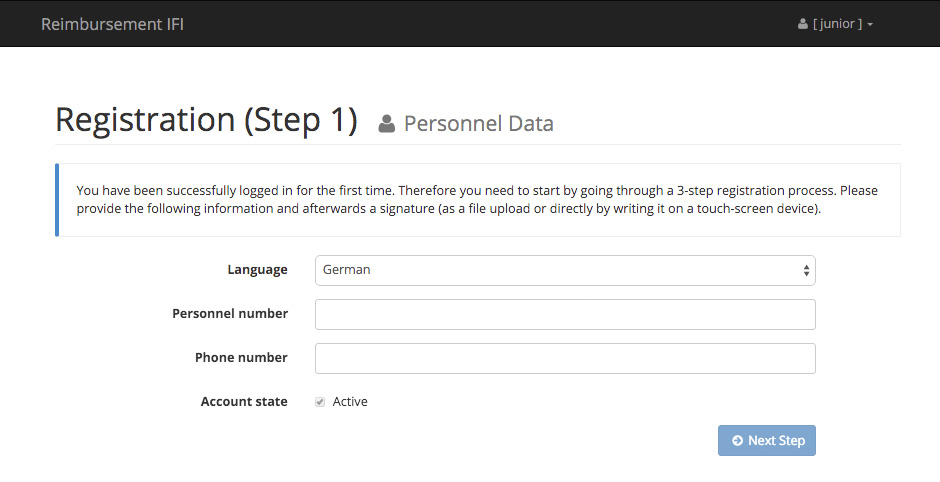
\includegraphics[width=0.80\textwidth]{registration-step01}}
    \caption{Registration step one: Capture personnel data}
    \label{fig:registration-step01}
\end{figure}

On Figure \ref{fig:registration-step02} the user has to add his signature either by uploading an image or capturing using a third party touchscreen device like a smart phone or try it in the browser. This signature is mandatory for the signature of the generated Pdf document containing all expense items.  

\begin{figure}[H]
    \centering
    \fbox{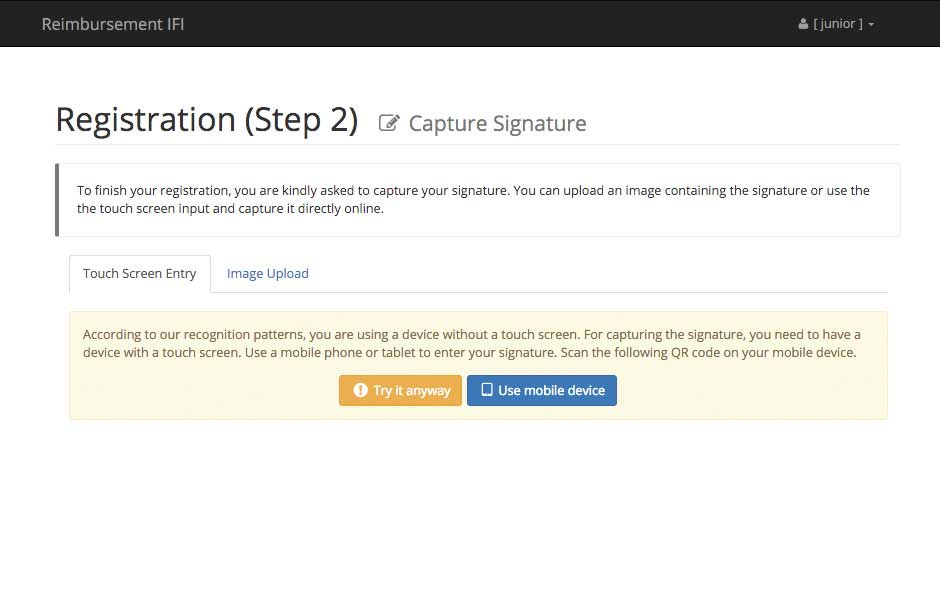
\includegraphics[width=0.80\textwidth]{registration-step02}}
    \caption{Registration step two: Capture signature}
    \label{fig:registration-step02}
\end{figure}

After completing the registration process, these captured information and signature can always be edited by going to the settings screen via the menu bar.
\clearpage

\section{Expenses}

An expense is an entity captured by the user. Every expense is defined by an \textbf{accounting description} that will be visual in SAP. An expense consists of 1 to 15 receipts. 

\begin{figure}[H]
    \centering
    \fbox{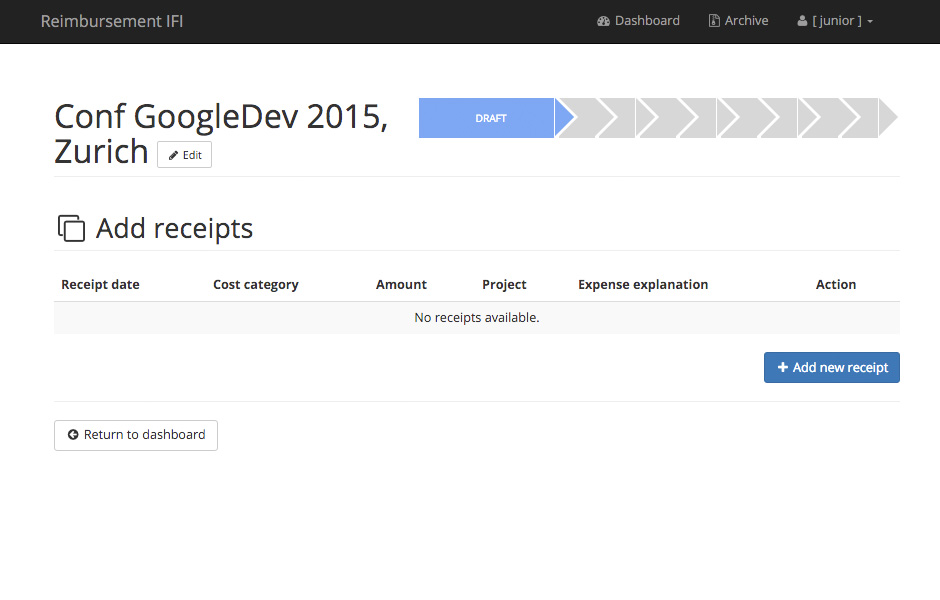
\includegraphics[width=0.80\textwidth]{expenses-add01}}
    \caption{Expense: Add new receipt}
    \label{fig:expenses-add01}
\end{figure}

A receipt consists out of the following mandatory fields (see Figure \ref{fig:expenses-add01}):
\begin{itemize}
    \item \textbf{Receipt date} will further be used to calculate the correct exchange rate if a foreign currency is selected.  
    \item \textbf{Cost category} selected out of a defined list of available cost categories.
    \item Original and calculated amount based on the exchange rate.
    \item The \textbf{project assignment} is added by a user with role \textit{manager}, \textit{deputy manager} or \textit{finance administrator}.
    \item A short \textbf{explanation} that describes the purpose of the receipt.   
    \item \textbf{Attachment} used for verification purpose of the captured receipt. 
\end{itemize}

Every expense will be in one of the following states during the process:

\begin{itemize}
    \item \textbf{DRAFT} status occurs if the expense is created and it has not been assigned to a \textit{manager}.
    \item \textbf{ASSIGNED} status occurs if a \textit{manager} or \textit{deputy manager} has assigned the expense to him.
    \item \textbf{REJECTED} status occurs if the created expense is not accepted by the \textit{manager}, \textit{deputy manager} or \textit{finance administrator}. In \textbf{REJECTED} status it will be reassigned to the user who created it.
    \item \textbf{SIGNED} status occurs if the expense has been signed by all three instances; \textit{employee}, \textit{manager} or \textit{deputy manager} and \textit{finance administrator}
    \item \textbf{PRINTED} status occurs if the expense and all its receipts are successfully converted into a digital document.
\end{itemize}

\section{User}

Every user that exists in the LDAP of the University of Zurich is capable to login to the system. He can use the same user name and password that he uses for the other University of Zurich services for login. See Section \ref{sec:registration} for more details.  

There exists different roles for users to login to the system. A user is allowed to have exactely one role out of the four defined. The roles are provided and synchronized with the LDAP-Server of the University of Zurich. The following roles exist in the system:

\begin{itemize}
    \item \textbf{Employees} are authorized to create and edit expenses that they created. However, an expense cannot be edited once it has been assigned to a manger.
    \item \textbf{Managers} are authorized to reject, accept and edit expenses that he assigns to him. A \textit{manager} is also capable of creating expenses and editing them until it has been assigned to a deputy manger.
    \item \textbf{Deputy manager} has the same authorizations as the \textit{manager} for designated \textit{managers} or if a \textit{manager} is outreach.   
    \item \textbf{Finance administrator} is authorized to reject, accept and edit expenses after they have been accepted by a \textit{manager} or \textit{deputy manager}. Furthermore they can manage the available cost categories.
\end{itemize}

\section{Guest view}

